\chapter{Oscillatore armonico}

\begin{equation*}
    H = \frac{p^2}{2m} + \underbrace{\frac{1}{2} m \omega^2}_k x^2
\end{equation*}
In prima approssimazione serve a risolvere molti problemi (intorno a punti di minimo) \newline
Potenziale oscillatore armonico è di tipo quadratico; intorno a un punto di minimo \( V'(x_0)=0 \) posso fare uno sviluppo in serie di Taylor
\begin{equation*}
    V(x) = V(x_0) + V(x_0)'(x-x_0) + \frac{1}{2}V''(x_0){(x-x_0)}^2
\end{equation*}
\begin{itemize}
    \item Vibrazioni atomi di una molecola
    \item Oscillazioni di atomi in reticolo cristallino \( \rightarrow\) FONONI
    \item Quantizzazione campo elettromagnetico \(\rightarrow\) FOTONI
\end{itemize}
Stati stazionari:
\begin{equation*}
    \left[-\frac{\hslash^2}{2m}\frac{d^2}{dx^2} + \frac{1}{2}m\omega^2 x^2  \right] \varphi(x) = E\varphi(x)
\end{equation*}
Essendo il potenziale di tipo quadratico, lo spettro dell'oscillatore armonico sarà discreto (2 punti di inversione del moto). \newline
Esistono 2 metodi di risoluzione:
\begin{itemize}
    \item Metodo standard: risoluzione equazione differenziale \newline
    Per prima cosa rendo l'espessione adimensionata 
    \begin{equation*}
        \xi = \frac{2E}{\hslash\omega} \tag{a}
    \end{equation*}
    allora l'equazione diventa
    \begin{equation*}
        \left(-\frac{\hslash}{m\omega} \frac{d^2}{dx^2} + \frac{m\omega}{\hslash} x^2\right)\varphi - \xi\varphi = 0 
    \end{equation*}
    introduco y
    \begin{equation*}
        y = \sqrt[]{\frac{m\omega}{\hslash}} x \qquad \frac{dy}{dx} = \sqrt[]{\frac{m\omega}{\hslash}} \qquad \frac{d}{dx} = \frac{dy}{dx} \frac{d}{dy}
    \end{equation*}
    otteniamo
    \begin{equation*}
        \frac{d^2}{dy^2} \varphi + (\xi - y^2)\varphi = 0 \tag{b}
    \end{equation*}
    Guardo cosa succede all'infinito (localmente decrescita esponenziale)
    \begin{equation*}
        y \to \pm \infty \Rightarrow \ddot{\varphi} - y^2 \simeq 0 \tag{1}
    \end{equation*}
    ipotizzando che 
    \begin{equation*}
        \varphi \div e^{-ay^2}
    \end{equation*}
    si ha che 
    \begin{equation*}
        \dot{\varphi} = -2aye^{-ay^2} \qquad \ddot{\varphi} = (-2a + 4a^2y^2) e^{-ay^2}
    \end{equation*}
    sostituendo nella (1) 
    \begin{gather*}
        (-2a + 4a^2y^2 - y^2) e^{-ay^2} \simeq 0 \\
        [-2a + (4a^2 - 1)y^2] e^{-ay^2} \simeq 0 \\
        4a^2 - 1 = 0 \Rightarrow a = \frac{1}{2}
    \end{gather*}
    Quindi
    \begin{equation*}
        \varphi(x) = e^{-\frac{y^2}{2}}h(x) \tag{**}
    \end{equation*}
    sostituendo (**) in (b) 
    \begin{equation*}
        \frac{d^2}{dy^2} h(y) - 2y \frac{dh(y)}{dy} + (\xi-1)h(y) = 0 \tag{2} 
    \end{equation*}
    Per \(y << \infty\)
    \begin{equation*}
        h(y) 0 \sum_{m=0}^\infty a_m y^m \tag{c}
    \end{equation*}
    sostituendo (c) in (2) ricavo il coefficiente di \(y^m\)
    \begin{equation*}
        (m+1)(m+2) a_{m+2} = (2m - \xi +1)a_m \tag{3}
    \end{equation*}
    \begin{itemize}
        \item \(a_0\): serie di soli termini pari
        \item \(a_2\): serie di soli termini dispari
    \end{itemize}
    Guardo il comportamento per m grande (\(m>N\))
    \begin{equation*}
        a_{m+2} \simeq \frac{2m}{m^2} a_m \simeq \frac{2}{m}a_m
    \end{equation*}
    allora la funzione \(h(y)\) ha un andamento polinomiale fino a N, poi
    \begin{equation*}
        a_Ny^N + \frac{2}{N} a_N y^{N+2} + \frac{2^2}{(N+2)N}a_N y^{N+4} + \frac{2^3}{(N+4)(N+2)N}a_N y^{N+6} + \dots 
    \end{equation*}
    \begin{equation*}
        h(y) = \dots + a_N y^2 \left(\frac{N}{2}\right)! \left[\frac{{(y^2)}^{\frac{N}{2}-1}}{\left(\frac{N}{2}-1\right)!} + \frac{{(y^2)}^{\frac{N}{2}}}{\left(\frac{N}{2}\right)!} + \frac{{(y^2)}^{\frac{N}{2}+1}}{\left(\frac{N}{2}+1\right)!}\right] \simeq \text{cost} y^2 [e^{y^2} - \text{polinomio in y}]         
    \end{equation*}
    \begin{equation*}
        h(y) \simeq \text{cost } y^2 e^{y^2} + \text{pol}
    \end{equation*}
    Da (**)
    \begin{equation*}
        \varphi \simeq e^{-\frac{y^2}{2}y^2e^{y^2}} \simeq y^2 e^{\frac{y^2}{2}}
    \end{equation*}
    che diverge per y grande; devo impedire che la serie mi dia esponenziale: la serie deve essere fermata \newline
    Se esiste n tale che 
    \begin{equation*}
        2n - \xi + 1 = 0 
    \end{equation*}
    allora la serie si ferma
    \begin{equation*}
        \xi = 2n + 1 \tag{d}
    \end{equation*}
    Sostituendo la (d) nella (a) ottengo che \textit{i livelli energetici devono essere quantizzati}
    \begin{equation*}
        E_n = \hslash \omega \left(n + \frac{1}{2}\right) \qquad n = 0,1,2, \dots 
    \end{equation*}
    Conseguenze:
    \begin{enumerate}
        \item Energia è quantizzata con pacchetti \(\hslash \omega \)
        \item Stato con energia minima (energia di punto 0)
        \begin{equation*}
            E_0 = \frac{\hslash\omega}{2}
        \end{equation*}
        in accordo con il principio di indeterminazione di Heisenberg
        \item Sostituendo (d) in (2) si ottiene l'equazione dei polinomi di Hermite
        \begin{equation*}
            \frac{d^2h}{dy^2} - 2y \frac{dh}{dy} + 2nh = 0
        \end{equation*}
    \end{enumerate}
    
    \item Metodo algebrico: Dirac
    \begin{gather*}
        \hat{H} = \frac{\hat{p}^2}{2m} + \frac{1}{2} m\omega^2x^2 \qquad [\hat{x},\hat{p}] = i\hslash \\        
        \hat{H}|\varphi> = E|\varphi>
    \end{gather*}
    Rendo le quantità adimensionate
    \begin{gather*}
        \hat{\tilde{x}} = \sqrt[]{\frac{m\omega}{\hslash}}\hat{x} \qquad \hat{\tilde{p}} = \frac{1}{\sqrt[]{m\hslash\omega}}\hat{p} \qquad \hat{\tilde{H}} = \frac{\hat{H}}{\hslash \omega}  \\
        [\hat{\tilde{x}}, \hat{\tilde{p}}] = i 
    \end{gather*}
    \begin{equation*}
        \hat{\tilde{H}} = \frac{1}{2}(\hat{\tilde{x}}^2 + \hat{\tilde{p}}^2) = \frac{\hat{\tilde{x}}+ i \hat{\tilde{p}}}{\sqrt[]{2}}\frac{\hat{\tilde{x}}- i \hat{\tilde{p}}}{\sqrt[]{2}} - \frac{1}{2}
    \end{equation*}
definisco
\begin{equation*}
    \tag{e}
    \begin{aligned}
        \hat{a} = \frac{1}{\sqrt[]{2}}(\hat{\tilde{x}}+ i\hat{\tilde{p}}) \quad \text{distruttore} \\
        \hat{a}^+ = \frac{1}{\sqrt[]{2}}(\hat{\tilde{x}}- i\hat{\tilde{p}}) \quad \text{costruttore}
    \end{aligned}
\end{equation*}
da (e) 
\begin{equation*}
    \hat{\tilde{x}} = \frac{1}{\sqrt[]{2}}(\hat{a}^++\hat{a}) \qquad \hat{\tilde{p}} = \frac{i}{\sqrt[]{2}}(\hat{a}^+-\hat{a})
\end{equation*}
\begin{equation*}
    [\hat{a},\hat{a}^+] = 1 \Rightarrow \hat{a}\hat{a}^+ -\hat{a}^+\hat{a} = 1 \tag{f}
\end{equation*}
usando la (f)
\begin{equation*}
    \hat{\tilde{H}} = \hat{a}\hat{a}^+ -\frac{1}{2} = \hat{a}^+\hat{a} + \frac{1}{2}
\end{equation*}
posso definire l'operatore numero
\begin{equation*}
    \hat{N} = \hat{a}^+\hat{a}
\end{equation*}
allora
\begin{equation*}
    \hat{\tilde{H}} = \hat{N} + \frac{1}{2}
\end{equation*}
N.B. \(\hat{N}\) è autoaggiunto
\begin{equation*}
    \hat{N}^+ = {(\hat{a}^+\hat{a})}^+ = \hat{a}^+\hat{a}
\end{equation*}
\begin{itemize}
    \item \([\hat{N},\hat{a}] = -\hat{a}\)
    \item \([\hat{N},\hat{a}^+] = \hat{a}^+\)
\end{itemize}
\end{itemize}

\section{Ricerca spettro di N}

\begin{gather*}
    \hat{N}|\nu> = \nu|\nu> \qquad <\nu|\nu> = 1 \; \nu\in \R \\
    \hat{H}|\nu> = \left(\nu + \frac{1}{2}\right)|\nu>
\end{gather*}
Calcolo
\begin{gather}
    \boxed{\hat{N}\hat{a}|\nu> = (\nu-1)\hat{a}|\nu>} \tag{4} \\
    \hat{N}\hat{a}^+ |\nu> = (\nu+1) \hat{a}^+|\nu> \tag{5}
\end{gather}
allora
\begin{itemize}
    \item \(\nu\) è autovalore corrispondente a \(\hat{N}|\nu>\)
    \item \((\nu+1)\) è autovalore corrispondente a \(\hat{a}^+|\nu>\)
    \item \((\nu-1)\) è autovalore corrispondente a \(\hat{a}|\nu>\)
\end{itemize}
Nello spazio di Hilbert, la norma è sempre maggiore o uguale a 0 ed nulla se e soltanto se il vettore è nullo
\begin{equation*}
    0 \leq {||a|\nu>||}^2 = <\nu|\hat{a}^+\hat{a}|\nu> = \nu <\nu|\nu> = \nu \qquad \Rightarrow \nu \geq 0
\end{equation*}
Conseguenze:
\begin{enumerate}
    \item Esiste un minimo \(\rightarrow \nu =0\) corrispondente allo stato \(|0>\); poichè la norma è nulla vale che \(a|0> = 0\): \textit{stato fondamentale}
    \begin{equation*}
        \hat{N}|0> = 0|0> 
    \end{equation*}
    \item \(\nu>0 \quad \nu \in \R \) \newline
    Applico la (4) \newline
    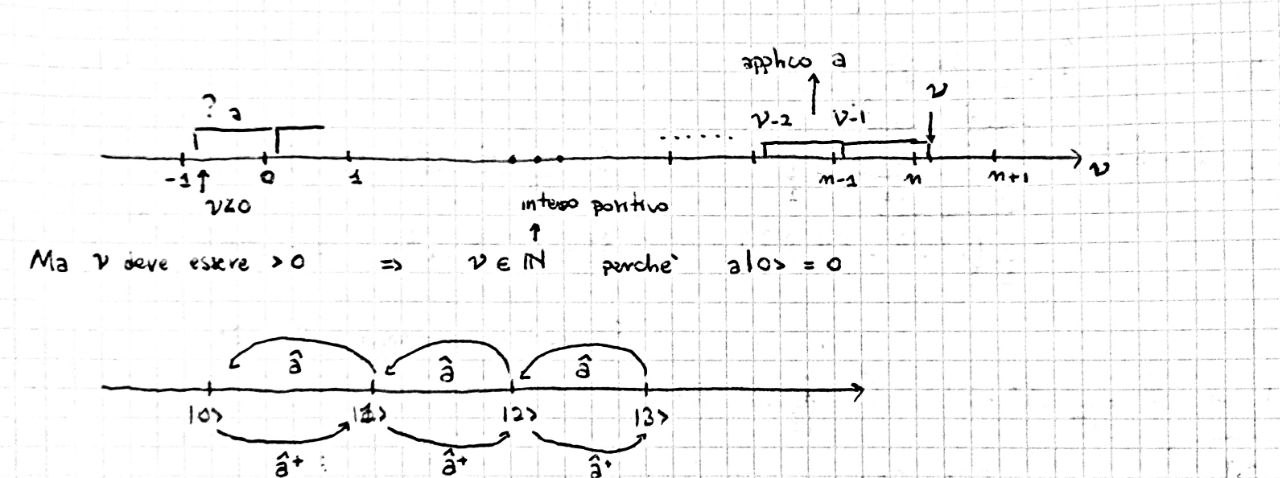
\includegraphics[width=\linewidth]{immagini/oscillatore_armonico1.jpg}
    Gli autovalori di \(\hat{N}\) appartengono ai numeri reali: ecco perchè del nome \textit{operatore numero}
\end{enumerate}

\section{Rappresentazione degli stati}

\begin{gather*}
    a|0> = 0 \\
    a^+a|0> \div |1> \\
    a^+|n> = c_n |n+1> \tag{c}
\end{gather*}
Ne calcolo la norma al quadrato di (c)
\begin{gather}
        {||a^+|n>||}^2 = \dots = (n+1) \tag{a} \\
        {||c_n|n+1>||}^2 = {|c_n|}^2 \tag{b}
\end{gather}
uguagliando (a)=(b)
\begin{equation*}
    {|c_n|}^2 = n+1 \Rightarrow c_n = \sqrt[]{n+1}
\end{equation*}
sostituendo nella (c)
\begin{equation*}
    a^+|n> = \sqrt[]{n+1} |n+1> \tag{6}
\end{equation*}
facendo i conti, si può anche ottenere
\begin{equation*}
    a|n> = \sqrt[]{n}|n-1> \tag{7}
\end{equation*}
usando la (6)
\begin{equation*}
    |n> = \frac{1}{\sqrt[]{n}}a^+|n-1>
\end{equation*}
Ripetendo 
\begin{equation*}
    |n> = \frac{1}{\sqrt[]{n!}} {(a^+)}^n |0> 
\end{equation*}

\section{Trovare rappresentazione dello stato fondamentale}

Riconverto a in termini di x e p
\begin{equation*}
    \frac{1}{\sqrt[]{2}}\left[\sqrt[]{\frac{m\omega}{\hslash}}\hat{x} + i \frac{1}{\sqrt[]{m\hslash\omega}}\hat{p}\right]|0> = 0 \tag{a}
\end{equation*}
\begin{enumerate}
    \item \(\hat{x}|x'> = x'|x'>\)
    \item \(<x|\hat{p} = -i\hslash \frac{d}{dx}<x|\)
\end{enumerate}
moltiplicando la (a) per \(<x|\) si ottiene
\begin{gather*}
    \left\{\sqrt[]{\frac{m\omega}{\hslash}}x + i \frac{1}{\sqrt[]{m\hslash\omega}}\left(-i\hslash\frac{d}{dx}\right)\right\}<x|0> = 0 \\
    \left(\frac{m\omega}{\hslash}x + \frac{d}{dx}\right) \varphi_0(x) = 0 
\end{gather*}
integrando e imponendo la condizione di normalizzazione 
\begin{equation*}
    \varphi_0 (x) = {\frac{m\omega}{\pi\hslash}}^{\frac{1}{4}} e^{-\frac{m\omega}{2\hslash}x^2} \tag{9}
\end{equation*}
Calcolo il bracket 
\begin{equation*}
    <x|n> = \varphi_n(x) = \frac{1}{\sqrt[]{n!}} \frac{1}{\sqrt[]{2^n}} {\left(\sqrt[]{\frac{m\omega}{\hslash}}x - \sqrt[]{\frac{\hslash}{m\omega}}\frac{d}{dx}\right)}^n \varphi_0(x)
\end{equation*}
introducendo
\begin{equation*}
    \xi = \sqrt[]{\frac{m\omega}{\hslash}}x
\end{equation*}
si trova
\begin{equation*}
    \varphi_n (x) = {\frac{m\omega}{\pi\hslash}}^{\frac{1}{4}} \frac{H_n(\xi)}{\sqrt[]{2^nn!}}e^{-\frac{\xi^2}{2}}
\end{equation*}
dove gli \(H_n(\xi)\) sono i polinomi di Hermite
\begin{equation*}
    H_n(\xi) = {(-1)}^n e^{\xi^2}{\left(\frac{d}{d\xi}\right)}^ne^{-\xi^2}
\end{equation*}

\section{Rappresentazione matriciale}

\begin{gather*}
    a^+|n> = \sqrt[]{n+1} |n+1> \\
    a|n> = \sqrt[]{n}|n-1> \\
    \hat{x}|n> = \sqrt[]{\frac{\hslash}{2m\omega}} (\sqrt[]{n+1} |n+1> + \sqrt[]{n}|n-1>) \\
    \hat{p} |n> = \sqrt[]{\frac{m\hslash\omega}{2}} (\sqrt[]{n+1} |n+1> - \sqrt[]{n}|n-1>)
\end{gather*}
\begin{itemize}
    \item \(<n'|a|n> = \sqrt[]{n}\delta_{n',n-1}\)
    \item \(<n'|a^+|n> = \sqrt[]{n+1}\delta_{n',n+1}\)
    \item \(<n'|x|n> = \sqrt[]{\frac{\hslash}{2m\omega}} (\sqrt[]{n+1}\delta_{n',n+1}  + \sqrt[]{n}\delta_{n',n-1})\)
    \item \(<n'|p|n> = \sqrt[]{\frac{m\hslash\omega}{2}} (\sqrt[]{n+1}\delta_{n',n+1}  - \sqrt[]{n}\delta_{n',n-1})\)
    \item \(<n'|N|n> = n \delta_{n',n}\)
\end{itemize}
\begin{gather*}
    \hat{a} \dot{=} \left[
    \begin{array}[]{cccc}
        0 & \sqrt[]{1} & 0 & 0 \\
        0 & 0 & \sqrt[]{2} & 0 \\
        0 & 0 & 0 & \sqrt[]{3}
    \end{array}\right] \qquad 
    \hat{a}^+ \dot{=} \left[
    \begin{array}[]{cccc}
        0 & 0 & 0 & 0 \\
        \sqrt[]{1} & 0 & 0 & 0 \\
        0 & \sqrt[]{2}& 0 & 0
    \end{array}\right] \\
    \hat{N} \dot{=} \left[
    \begin{array}[]{cccc}
        1 & 0 & 0 & 0 \\
        0 & 2 & 0 & 0 \\
        0 & 0 & 3 & 0 \\
        0 & 0 & 0 & 4
    \end{array}\right] \\
    \hat{x} \dot{=} \, \sqrt[]{\frac{\hslash}{2m\omega}}\left[
    \begin{array}[]{cccc}
        0 & \sqrt[]{1} & 0 & 0 \\
        \sqrt[]{1} & 0 & \sqrt[]{2} & 0 \\
        0 & \sqrt[]{2}& 0 & \sqrt[]{3} \\
        0 & 0 & \sqrt[]{3} & 0 
    \end{array}\right] \qquad 
    \hat{p} \dot{=} \,  \sqrt[]{\frac{m\hslash\omega}{2}}\left[
    \begin{array}[]{ccc}
        0 & -i\, \sqrt[]{1} & 0 \\
        +i\, \sqrt[]{1} & 0 & -i \, \sqrt[]{2}  \\
        0 & i\, \sqrt[]{2}& 0  
    \end{array}\right]
\end{gather*}

\section{Oscillatore armonico 3D}

\boxedeq{\hat{H} = \hat{H}_x + \hat{H}_y + \hat{H}_z = \sum_{i=0}^3 -\frac{\hslash^2}{2m}\frac{\delta^2}{\delta x^2_i} + \frac{1}{2} m \omega^2_i x^2_i}
\begin{equation*}
    \varphi (x,y,z) = \varphi^{\omega_1}_{n_1}(x) + \varphi^{\omega_2}_{n_2}(y) + \varphi^{\omega_3}_{n_3}(z)
\end{equation*}
\begin{equation*}
     E_{n_1,n_2,n_3} = \hslash\omega_1 \bra{n_1 + \frac{1}{2}} + \hslash\omega_2 \bra{n_2 + \frac{1}{2}} + \hslash\omega_3 \bra{n_3 + \frac{1}{2}}
\end{equation*}
Se \(\omega_1,\omega_2,\omega_3\) sono incommensurabili \(\Rightarrow\) non c'è degenerazione \newline
Posso aumentare al massimo la simmetria: \(\omega = \omega_1 = \omega_2 = \omega_3\)
\begin{equation*}
    \hat{H} = \frac{\hat{p}^2}{2m} + \frac{1}{2} m \omega^2 \hat{\vec{x}}^2 \qquad V = \frac{1}{2}m\omega^2r^2 = V(r) \mbox{ sferosimmetrico}
\end{equation*}
allora nascono nuove costanti del moto e quindi compare la degenarazione
\begin{gather*}
    E_{n_1,n_2,n_3} = \hslash\omega \bra{n_1 + n_2 + n_3 + \frac{3}{2}} \\
    n_{deg} = \frac{1}{2}(n+1)(n+2) \qquad n = n_1 + n_2 + n_3
\end{gather*}
